\subsection{Sistema de coordenadas}
É conveniente utilizar um sistema de coordenadas cilíndrico para descrever a trajetória de um elétron dentro do anel de armazenamento (\autoref{fig:fig7}), uma vez que é desejado que seu movimento seja circular. Sendo assim, definem-se as coordenadas
\begin{itemize}
	\item $s$ -- Coordenada longitudinal, representa a distância entre um ponto de referência na órbita ideal e o ponto mais próximo do elétron nesta mesma órbita.
	\item $x$ e $z$ -- Coordenadas transversais, representam os deslocamentos horizontal e vertical com relação à órbita ideal, respectivamente.
\end{itemize}

\begin{figure}[!htb]
	\centering
	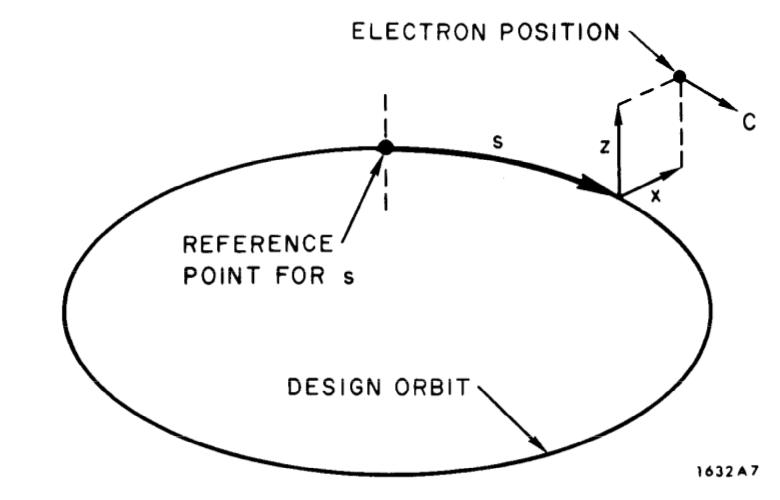
\includegraphics[width=0.6\linewidth]{./Figuras/fig7.jpeg}
	\caption{Coordenadas para descrever as trajetórias. Retirado de \cite{sands1970physics}.}
	\label{fig:fig7}
\end{figure}